\documentclass[12pt]{article}
%^ Start of document
\usepackage{times}  %Makes text TimesNewRoman
\usepackage{setspace} %Allows you to set single or double space 
\usepackage{biblatex} %Imports biblatex package
\usepackage{graphicx} % Required for inserting images
\usepackage{authblk}
\usepackage[colorlinks=true, urlcolor=blue, linkcolor=blue]{hyperref}
\usepackage{subfig}
\usepackage{float}
\usepackage{tabularx}
\usepackage{multirow}
\usepackage[paperheight=11in,
   paperwidth=8.5in,
   top=20mm,
   bottom=20mm,
   left=40mm,
   right=40mm]{geometry}
\usepackage{moresize}
\usepackage{tikz}
\usepackage{xcolor}
\usepackage{physics}
\usepackage{amssymb}
\usepackage{mathrsfs}
\usepackage{amsmath}
\usepackage[document]{ragged2e}
\usepackage{comment}
\usepackage{xcolor}
\addbibresource{Qhw.bib}
\begin{document}
\singlespacing  %Sets single spacing for whole document
\title{Quantum Final HW}

\author[1]{Zachary Tullier}
\affil[1]{Student\\Physics Department\\ University of Houston - Clear Lake \\Houston, Texas\\U.S}
\date{}
\maketitle

\section{Question 1}
    \begin{itemize}
        \item [(a)] A particle is initially in its ground state in a one-dimensional harmonic oscillator potential,
        \[
            V(x) = \frac{1}{2} k x^2.
        \]
        If the spring constant is suddenly doubled, calculate the probability of finding the particle in the ground state of the new potential.
        \item [(b)] Show how a vector operator \( A \) transforms under a rotation of angle \( \alpha \) about the \( y \)-axis.
        \item [(c)] Show how \( J_x \) and \( J_y \) transform under a rotation of (finite) angle \( \varphi \) about the \( z \)-axis. Using these results, determine how the angular momentum operator \( \vec{J} \) transforms under the rotation.
        \item [(d)] Construct all the spin states with \( n = 3 \), \( \ell = 0, 1, 2 \). Find out the corresponding value of \( \vec{L} \cdot \vec{S} \) of each state. How do \( L \)-\( S \) couplings contribute to the total angular momentum \( \vec{J} \)?
    \end{itemize}

    \subsection{Solution, part (a):}
        We are given:
        \[
            V(x) = \frac{1}{2} kx^2
        \]
        Initially, the system is in the ground state of this potential. The spring constant is suddenly doubled: \( k \to 2k \). We are to compute the probability that the particle is found in the ground state of the new potential.
        
        Let:
        \[
            \omega_1 = \sqrt{\frac{k}{m}}, \quad \omega_2 = \sqrt{\frac{2k}{m}} = \sqrt{2} \omega_1
        \]
        
        The ground state wavefunction of a 1D harmonic oscillator is:
        \[
            \psi_0^{(\omega)}(x) = \left( \frac{m \omega}{\pi \hbar} \right)^{1/4} \exp\left( - \frac{m \omega x^2}{2\hbar} \right)
        \]
        
        Then:
        \[
            \psi_{\text{initial}} = \psi_0^{(\omega_1)}(x), \quad
            \psi_{\text{final}} = \psi_0^{(\omega_2)}(x)
        \]
        
        The overlap (transition) probability is:
        \[
            P = \left| \int_{-\infty}^{\infty} \psi_0^{(\omega_2)}(x)^* \psi_0^{(\omega_1)}(x) \, dx \right|^2
        \]
        
        Evaluating the Gaussian integral:
        \[
            I = \int_{-\infty}^{\infty}
            \left( \frac{m \omega_2}{\pi \hbar} \right)^{1/4}
            \left( \frac{m \omega_1}{\pi \hbar} \right)^{1/4}
            \exp\left[ - \frac{m}{2\hbar} (\omega_1 + \omega_2) x^2 \right] dx
        \]
        
        Using the standard Gaussian integral:
        \[
            \int_{-\infty}^{\infty} e^{-a x^2} dx = \sqrt{\frac{\pi}{a}}, \quad \text{for } a > 0
        \]
        
        We find:
        \[
            I = \left( \frac{4 \omega_1 \omega_2}{(\omega_1 + \omega_2)^2} \right)^{1/4}
            \Rightarrow
            P = \left( \frac{4 \omega_1 \omega_2}{(\omega_1 + \omega_2)^2} \right)^{1/2}
        \]
        
        Substitute \( \omega_2 = \sqrt{2} \omega_1 \):
        \[
            P = \left( \frac{4 \omega_1 \sqrt{2} \omega_1}{\left( \omega_1 + \sqrt{2} \omega_1 \right)^2} \right)^{1/2}
            = \left( \frac{4\sqrt{2}}{(1 + \sqrt{2})^2} \right)^{1/2}
            = \frac{2^{3/4}}{1 + \sqrt{2}} \approx \boldsymbol{\boxed{0.84}}
        \]

    \subsection{Solution, part (b):}
        Let \( \vec{A} \) be a vector operator. Under a rotation of angle \( \alpha \) about the \( y \)-axis, the components transform as:
        \[
            A'_i = R_{ij}(\alpha) A_j
        \]
        
        The rotation matrix about the \( y \)-axis is:
        \[
            R_y(\alpha) =
            \begin{pmatrix}
                \cos \alpha & 0 & \sin \alpha \\
                0 & 1 & 0 \\
                - \sin \alpha & 0 & \cos \alpha
            \end{pmatrix}
        \]
        
        So,
        \[
            \begin{aligned}
                A_x' &= A_x \cos \alpha + A_z \sin \alpha \\
                A_y' &= A_y \\
                A_z' &= -A_x \sin \alpha + A_z \cos \alpha
            \end{aligned}
        \]
        
    \subsection{Solution, part (c):}
        A rotation by angle \( \varphi \) about the \( z \)-axis is generated by:
        \[
            U(\varphi) = e^{-i \varphi J_z / \hbar}
        \]
        
        The operators transform as:
        \[
            J'_x = U^\dagger J_x U, \quad J'_y = U^\dagger J_y U
        \]
        
        Using the commutation relations:
        \[
            [J_z, J_x] = i \hbar J_y, \quad [J_z, J_y] = -i \hbar J_x
        \]
        
        One obtains:
        \[
            \begin{aligned}
                J_x' &= J_x \cos \varphi + J_y \sin \varphi \\
                J_y' &= -J_x \sin \varphi + J_y \cos \varphi \\
                J_z' &= J_z
            \end{aligned}
        \]
        
        Thus, \( \vec{J} \) transforms like a vector under rotations.

    \subsection{Solution, part (d):}
        We are given:
        \[
            n = 3, \quad \ell = 0, 1, 2, \quad s = \frac{1}{2}
        \]
        
        For each \( \ell \), possible total angular momentum quantum numbers are:
        \[
            j = \ell \pm \frac{1}{2}
        \]
        
        The operator \( \vec{L} \cdot \vec{S} \) has eigenvalue:
        \[
            \vec{L} \cdot \vec{S} = \frac{1}{2} \left[ J(J+1) - L(L+1) - S(S+1) \right] \hbar^2
        \]
        
        Case \( \ell = 0 \):
        \[
            j = \frac{1}{2} \Rightarrow \vec{L} \cdot \vec{S} = \frac{1}{2} \left( \frac{3}{4} - 0 - \frac{3}{4} \right) \hbar^2 = 0
        \]
        
        Case \( \ell = 1 \):
        \[
            \begin{aligned}
                j = \frac{1}{2} &\Rightarrow \vec{L} \cdot \vec{S} = \frac{1}{2} \left( \frac{3}{4} - 2 - \frac{3}{4} \right) \hbar^2 = -\hbar^2 \\
                j = \frac{3}{2} &\Rightarrow \vec{L} \cdot \vec{S} = \frac{1}{2} \left( \frac{15}{4} - 2 - \frac{3}{4} \right) \hbar^2 = \frac{5}{4} \hbar^2
            \end{aligned}
        \]
        
        Case \( \ell = 2 \):
        \[
            \begin{aligned}
                j = \frac{3}{2} &\Rightarrow \vec{L} \cdot \vec{S} = \frac{1}{2} \left( \frac{15}{4} - 6 - \frac{3}{4} \right) \hbar^2 = -\frac{3}{2} \hbar^2 \\
                j = \frac{5}{2} &\Rightarrow \vec{L} \cdot \vec{S} = \frac{1}{2} \left( \frac{35}{4} - 6 - \frac{3}{4} \right) \hbar^2 = \frac{5}{2} \hbar^2
            \end{aligned}
        \]


\section{Question 2}
\begin{itemize}
    \item [(a)] Prove that \( J^2 \) and \( J_z \) are the eigenvalue operators whereas \( J_x \) and \( J_y \) are not the eigenvalue operators. Also show that
    \[
        \hat{J}_{\pm} \ket{j, m} = \hbar \sqrt{j(j+1) - m(m \pm 1)} \ket{j, m \pm 1}
    \]
    or equivalently,
    \[
        \hat{J}_{\pm} \ket{j, m} = \hbar \sqrt{(j \mp m)(j \pm m + 1)} \ket{j, m \pm 1}
    \]
    \item [(b)] Show that
    \[
        e^{i \hat{J}_z \phi / \hbar} e^{i \alpha \hat{J}_y / \hbar} e^{-i \hat{J}_z \phi / \hbar} = e^{i \alpha \hat{J}_y' / \hbar}
    \]
\end{itemize}

    \subsection{Solution, part (a):}
        The angular momentum eigenstates \( \ket{j, m} \) satisfy:
        \[
            \hat{J}^2 \ket{j, m} = \hbar^2 j(j+1) \ket{j, m}, \qquad
            \hat{J}_z \ket{j, m} = \hbar m \ket{j, m}
        \]
        
        Thus, \( \hat{J}^2 \) and \( \hat{J}_z \) are diagonal in this basis and are eigenvalue operators. We define the ladder operators:
        \[
            \hat{J}_\pm = \hat{J}_x \pm i \hat{J}_y
        \]
        
        which implies:
        \[
            \hat{J}_x = \frac{1}{2}(\hat{J}_+ + \hat{J}_-), \qquad \hat{J}_y = \frac{1}{2i}(\hat{J}_+ - \hat{J}_-)
        \]
        
        These operators change the value of \( m \):
        \[
            \hat{J}_\pm \ket{j, m} \propto \ket{j, m \pm 1}
        \]
        
        Thus, neither \( \hat{J}_x \) nor \( \hat{J}_y \) has \( \ket{j, m} \) as eigenstates—they are not eigenvalue operators in this basis. Now, let’s derive the action of the ladder operators. We use the commutation relations:
        \[
            [\hat{J}_z, \hat{J}_\pm] = \pm \hbar \hat{J}_\pm, \qquad [\hat{J}_+, \hat{J}_-] = 2\hbar \hat{J}_z
        \]
        
        and:
        \[
            \hat{J}^2 = \hat{J}_z^2 + \frac{1}{2}(\hat{J}_+ \hat{J}_- + \hat{J}_- \hat{J}_+)
        \]
        
        Using these relations, we can derive:
        \[
            \hat{J}_\pm \ket{j, m} = \hbar \sqrt{j(j+1) - m(m \pm 1)} \ket{j, m \pm 1}
        \]
        
        Alternatively, this can be written as:
        \[
            \hat{J}_\pm \ket{j, m} = \hbar \sqrt{(j \mp m)(j \pm m + 1)} \ket{j, m \pm 1}
        \]
        
        Both expressions are equivalent and describe the ladder operation.

    \subsection{Solution, part (b):}
        We are to prove:
        \[
            e^{i \hat{J}_z \phi / \hbar} e^{i \alpha \hat{J}_y / \hbar} e^{-i \hat{J}_z \phi / \hbar} = e^{i \alpha \hat{J}_y' / \hbar}
        \]
        where \( \hat{J}_y' \) is the rotated operator.
        
        This is a standard operator conjugation (rotation) identity. Define the transformation:
        \[
            \hat{O}' = e^{i \hat{J}_z \phi / \hbar} \hat{O} e^{-i \hat{J}_z \phi / \hbar}
            \Rightarrow \hat{O}' \text{ is the operator rotated about the } z\text{-axis by angle } \phi
        \]
        
        Apply this to \( \hat{J}_y \):
        \[
            e^{i \hat{J}_z \phi / \hbar} \hat{J}_y e^{-i \hat{J}_z \phi / \hbar} = \hat{J}_y'
        \]
        
        Then the full identity becomes:
        \[
            e^{i \hat{J}_z \phi / \hbar} e^{i \alpha \hat{J}_y / \hbar} e^{-i \hat{J}_z \phi / \hbar} 
            = e^{i \alpha \hat{J}_y' / \hbar}
        \]
        
        This follows from the general identity:
        \[
            U A U^\dagger = A' \Rightarrow U e^{i \alpha A} U^\dagger = e^{i \alpha A'}
        \]
        
        \[
        \boxed{
            e^{i \hat{J}_z \phi / \hbar} e^{i \alpha \hat{J}_y / \hbar} e^{-i \hat{J}_z \phi / \hbar} = e^{i \alpha \hat{J}_y' / \hbar}        }
        \]

\section{Question 3}
    Consider a hydrogen atom which is subject to two \textit{weak} static fields: an electric field in the \( xy \) plane \( \vec{\mathcal{E}} = \mathcal{E}(\hat{i} + \hat{j}) \) and a magnetic field along the \( z \)-axis \( \vec{B} = B \hat{k} \), where \( \mathcal{E} \) and \( B \) are constant. Neglecting the spin–orbit interaction, calculate the energy levels of the \( n = 2 \) states to first-order perturbation.

    \subsection{Solution:}
        We are given:
        \begin{itemize}
            \item Hydrogen atom with principal quantum number \( n = 2 \)
            \item Weak electric field \( \vec{\mathcal{E}} = \mathcal{E}(\hat{i} + \hat{j}) \)
            \item Weak magnetic field \( \vec{B} = B \hat{k} \)
            \item Neglect spin–orbit interaction
            \item Use first-order perturbation theory
        \end{itemize}
        
        We must find the energy shifts of the \( n = 2 \) states due to both fields. In hydrogen with degeneracy of \( n = 2 \)
        \begin{itemize}
            \item \( n = 2 \Rightarrow \ell = 0, 1 \)
            \item For \( \ell = 0 \): \( m = 0 \)
            \item For \( \ell = 1 \): \( m = -1, 0, 1 \)
        \end{itemize}
        
        So there are 4 degenerate states:
        \[
            \ket{200}, \quad \ket{210}, \quad \ket{211}, \quad \ket{21{-1}}
        \]
        
        The following is the Stark Effect. The perturbation is:
        \[
            H_E = -e \vec{\mathcal{E}} \cdot \vec{r} = -e \mathcal{E} (x + y)
        \]
        
        In spherical coordinates:
        \[
            x + y = r \sin\theta (\cos\phi + \sin\phi)
            \Rightarrow H_E = -e \mathcal{E} r \sin\theta (\cos\phi + \sin\phi)
        \]
        
        This operator connects \( \ell = 0 \leftrightarrow \ell = 1 \) states with \( \Delta m = \pm 1 \), i.e., couples \( \ket{200} \leftrightarrow \ket{21,\pm1} \)
        
        The following is the Zeeman Effect. With no spin and weak field:
        \[
            H_B = \mu_B B \frac{\hat{L}_z}{\hbar}
            \Rightarrow H_B \ket{n\ell m} = \mu_B B m \ket{n\ell m}
        \]
        
        Only the \( \ell = 1 \) states are shifted:
        \[
            \Delta E = \mu_B B m
        \]
        
        Define the basis:
        \[
            \begin{aligned}
                &\ket{1} = \ket{200}, \\
                &\ket{2} = \ket{21{-1}}, \\
                &\ket{3} = \ket{210}, \\
                &\ket{4} = \ket{211}
            \end{aligned}
        \]
        
        Let \( a = \mel{21{-1}}{H_E}{200} = \mel{211}{H_E}{200} \). The total perturbation Hamiltonian is:
        \[
            H^{(1)} =
            \begin{pmatrix}
                0 & a & 0 & a \\
                a & -\mu_B B & 0 & 0 \\
                0 & 0 & 0 & 0 \\
                a & 0 & 0 & \mu_B B
            \end{pmatrix}
        \]
        
        Restricting to the 3-dimensional subspace \( \{ \ket{200}, \ket{21{-1}}, \ket{211} \} \), we have:
        \[
            H =
            \begin{pmatrix}
                0 & a & a \\
                a & -\mu_B B & 0 \\
                a & 0 & \mu_B B
            \end{pmatrix}
        \]
        
        To find the energy corrections, solve:
        \[
            \det(H - E I) = 0 \Rightarrow
            \begin{vmatrix}
                -E & a & a \\
                a & -\mu_B B - E & 0 \\
                a & 0 & \mu_B B - E
            \end{vmatrix} = 0
        \]
        
        Computing this determinant:
        \[
            -E \left[ (-\mu_B B - E)(\mu_B B - E) \right]
            - a^2(-\mu_B B - E)
            - a^2(\mu_B B - E)
            = 0
        \]
        
        This results in a cubic equation in \( E \), whose roots give the energy levels to first-order perturbation theory.

\section{Question 4}
    Consider a system which is in the state
    \[
        \psi(\theta, \varphi) = \sqrt{\frac{2}{13}} Y_{3,-3} + \sqrt{\frac{3}{13}} Y_{3,-2} + \sqrt{\frac{3}{13}} Y_{3,0} + \sqrt{\frac{3}{13}} Y_{3,2} + \sqrt{\frac{2}{13}} Y_{3,3}
    \]

    \begin{enumerate}
        \item[(a)] If \( \hat{L}_x \) were measured, what values will one obtain and with what probabilities?
        
        \item[(b)] If after a measurement of \( \hat{L}_z \) we find \( l_z = 2\hbar \), calculate the uncertainties \( \Delta L_x \) and \( \Delta L_y \), and their product \( \Delta L_x \Delta L_y \).
        
        \item[(c)] Find \( \langle \psi | \hat{L}_x | \psi \rangle \) and \( \langle \psi | \hat{L}_y | \psi \rangle \).
    \end{enumerate}

    \subsection{Solution, part (a):}
        Consider a system in the state:
        \[
            \psi(\theta, \varphi) = \sqrt{\frac{2}{13}} Y_{3,-3} + \sqrt{\frac{3}{13}} Y_{3,-2} + \sqrt{\frac{3}{13}} Y_{3,0} + \sqrt{\frac{3}{13}} Y_{3,2} + \sqrt{\frac{2}{13}} Y_{3,3}
        \]
        
        The operator \( \hat{L}_x \) does not commute with \( \hat{L}_z \), so the \( Y_{\ell m} \) basis is not an eigenbasis of \( \hat{L}_x \). We can write:
        \[
            \hat{L}_x = \frac{1}{2} \left( \hat{L}_+ + \hat{L}_- \right)
        \]
        
        This operator mixes states with \( m \to m \pm 1 \). Therefore, the spherical harmonics are not eigenstates of \( \hat{L}_x \), and one would need to express the state in terms of the \( \hat{L}_x \) eigenbasis to find exact measurement probabilities. However, the eigenstates of \( \hat{L}_x \) are not trivial to write in closed form, so we instead state:
        \begin{itemize}
            \item \( \hat{L}_x \) has eigenvalues ranging from \( -\hbar \sqrt{\ell(\ell+1)} \) to \( \hbar \sqrt{\ell(\ell+1)} \)
            \item The outcomes will lie within this spectrum
            \item Exact probabilities require diagonalizing \( \hat{L}_x \), which is nontrivial in this basis
        \end{itemize}
        
        We do not compute exact probabilities here, but this motivates parts (b) and (c).

    \subsection{Solution, part (b):}
        Given a measurement of \( \hat{L}_z \) yielding \( l_z = 2\hbar \), compute \( \Delta L_x \), \( \Delta L_y \), and their product

        Let the state be \( \ket{3,2} \). Then:
        \[
            \hat{L}_z \ket{3,2} = 2\hbar \ket{3,2}
        \]
        
        We know:
        \[
            \ev{\hat{L}_x} = \ev{\hat{L}_y} = 0 \quad \text{(since they shift \( m \), but diagonal terms vanish)}
        \]
        
        Thus:
        \[
            (\Delta L_x)^2 = \ev{\hat{L}_x^2}, \quad (\Delta L_y)^2 = \ev{\hat{L}_y^2}
        \]
        
        Using:
        \[
            \hat{L}^2 = \hat{L}_x^2 + \hat{L}_y^2 + \hat{L}_z^2 \Rightarrow \hat{L}_x^2 + \hat{L}_y^2 = \hat{L}^2 - \hat{L}_z^2
        \]
        
        Apply to \( \ket{3,2} \):
        \[
            \begin{aligned}
                \hat{L}^2 \ket{3,2} &= \hbar^2 \cdot 3(3+1) = 12\hbar^2 \\
                \hat{L}_z^2 \ket{3,2} &= (2\hbar)^2 = 4\hbar^2 \\
                \Rightarrow \ev{\hat{L}_x^2 + \hat{L}_y^2} &= 8\hbar^2
            \end{aligned}
        \]
        
        By symmetry:
        \[
            \ev{\hat{L}_x^2} = \ev{\hat{L}_y^2} = 4\hbar^2
            \Rightarrow \Delta L_x = \Delta L_y = 2\hbar, \quad \Delta L_x \Delta L_y = 4\hbar^2
        \]
        \[
            \boldsymbol{\boxed{\Delta L_x = 2\hbar, \quad \Delta L_y = 2\hbar, \quad \Delta L_x \Delta L_y = 4\hbar^2}}
        \]

    \subsection{Solution, part (c):}
        Compute \( \ev{\psi | \hat{L}_x | \psi} \) and \( \ev{\psi | \hat{L}_y | \psi} \)

        Use:
        \[
            \hat{L}_x = \frac{1}{2}(\hat{L}_+ + \hat{L}_-), \quad \hat{L}_y = \frac{1}{2i}(\hat{L}_+ - \hat{L}_-)
        \]
        \[
            \hat{L}_\pm \ket{\ell, m} = \hbar \sqrt{(\ell \mp m)(\ell \pm m + 1)} \ket{\ell, m \pm 1}
        \]
        
        The state:
        \[
            \psi = \sum_{m \in \{-3, -2, 0, 2, 3\}} c_m \ket{3, m}
        \]
        
        with:
        \[
            c_{-3} = \sqrt{\frac{2}{13}}, \quad
            c_{-2} = \sqrt{\frac{3}{13}}, \quad
            c_0 = \sqrt{\frac{3}{13}}, \quad
            c_2 = \sqrt{\frac{3}{13}}, \quad
            c_3 = \sqrt{\frac{2}{13}}
        \]
        
        Then:
        \[
            \ev{\hat{L}_x} = \sum_{m} c_m^* c_{m+1} \frac{\hbar}{2} \sqrt{(3 - m)(3 + m + 1)} + \text{c.c.}
        \]
        
        Terms with $m = -3$
        \[
            m = -3 \Rightarrow c_{-3}^* c_{-2} = \sqrt{\frac{6}{169}}, \quad \sqrt{6 \cdot 1} = \sqrt{6}
            \Rightarrow \text{contribution} = \frac{6\hbar}{2 \cdot 13} = \frac{3\hbar}{13}
        \]
        
        Same for \( m = 2 \to 3 \), total:
        \[
            \ev{\hat{L}_x} = \frac{3\hbar}{13} + \frac{3\hbar}{13} = \frac{6\hbar}{13}
        \]
        
        For \( \hat{L}_y \), the contributions are purely imaginary and symmetric:
        \[
            \Rightarrow \ev{\hat{L}_y} = 0
        \]
        
        \[
            \boldsymbol{\boxed{\begin{aligned}
            \ev{\hat{L}_x} &= \frac{6\hbar}{13} \\
            \ev{\hat{L}_y} &= 0
            \end{aligned}}}
        \]

\section{Question 5}
    Write the Schrödinger equation in spherical polar coordinates and write its solution as:
    \[
        \psi(\vec{r}) = \langle \vec{r} \mid n l m \rangle = \psi_{nlm}(r, \theta, \varphi) = R_{nl}(r) Y_{lm}(\theta, \varphi)
    \]
    
    Explicitly show how each of the special functions is a solution of the radial and angular components of the wavefunction that satisfies the corresponding Schrödinger equation.

    \subsection{Solution:}
        Write the Schrödinger equation in spherical polar coordinates and write its solution as:
        \[
            \psi(\vec{r}) = \braket{\vec{r} | n\ell m} = \psi_{n\ell m}(r, \theta, \varphi) = R_{n\ell}(r) Y_{\ell m}(\theta, \varphi)
        \]
        
        Explicitly show how each of the special functions is a solution of the radial and angular components of the wavefunction that satisfies the corresponding Schrödinger equation. For a central potential \( V(r) \) (e.g., the Coulomb potential \( V(r) = -\frac{e^2}{4\pi \varepsilon_0 r} \)), the time-independent Schrödinger equation is:
        \[
            \hat{H} \psi(\vec{r}) = E \psi(\vec{r}), \quad \text{where} \quad \hat{H} = -\frac{\hbar^2}{2\mu} \nabla^2 + V(r)
        \]
        
        The Laplacian in spherical coordinates \( (r, \theta, \varphi) \) is:
        \[
            \nabla^2 = \frac{1}{r^2} \frac{\partial}{\partial r} \left( r^2 \frac{\partial}{\partial r} \right)
            + \frac{1}{r^2 \sin \theta} \frac{\partial}{\partial \theta} \left( \sin \theta \frac{\partial}{\partial \theta} \right)
            + \frac{1}{r^2 \sin^2 \theta} \frac{\partial^2}{\partial \varphi^2}
        \]
        
        Assume a separable solution of the form:
        \[
            \psi(r, \theta, \varphi) = R_{n\ell}(r) Y_{\ell m}(\theta, \varphi)
        \]
        
        Substitute into the Schrödinger equation:
        
        \[
            -\frac{\hbar^2}{2\mu} \left[
            \frac{1}{r^2} \frac{d}{dr} \left( r^2 \frac{dR}{dr} \right) Y_{\ell m}
            + \frac{R}{r^2} \hat{L}^2 Y_{\ell m}
            \right] + V(r) R Y_{\ell m} = E R Y_{\ell m}
        \]
        
        Divide both sides by \( R Y_{\ell m} \), and multiply through by \( r^2 \), we obtain:
        
        \[
            -\frac{\hbar^2}{2\mu} \left[
            \frac{1}{R} \frac{d}{dr} \left( r^2 \frac{dR}{dr} \right)
            + \frac{1}{Y_{\ell m}} \hat{L}^2 Y_{\ell m}
            \right] + V(r) = E
        \]
        
        This leads to separation into two independent equations: one for \( R(r) \), and one for \( Y_{\ell m}(\theta, \varphi) \).
        
        The angular part of the Laplacian leads to:
        \[
            \hat{L}^2 Y_{\ell m}(\theta, \varphi) = \hbar^2 \ell(\ell + 1) Y_{\ell m}(\theta, \varphi)
        \]
        
        So the angular wavefunctions are the spherical harmonics, which satisfy:
        \[
            \left[
            \frac{1}{\sin \theta} \frac{\partial}{\partial \theta} \left( \sin \theta \frac{\partial}{\partial \theta} \right)
            + \frac{1}{\sin^2 \theta} \frac{\partial^2}{\partial \varphi^2}
            \right] Y_{\ell m} = -\ell(\ell + 1) Y_{\ell m}
        \]
        
        Substituting the angular solution into the radial part gives:
        
        \[
            -\frac{\hbar^2}{2\mu} \left[
            \frac{d^2 R}{dr^2} + \frac{2}{r} \frac{dR}{dr} - \frac{\ell(\ell + 1)}{r^2} R
            \right] + V(r) R = E R
        \]
        
        Or equivalently:
        \[
            \boldsymbol{\boxed{\frac{d^2 R}{dr^2} + \frac{2}{r} \frac{dR}{dr} + \left[
            \frac{2\mu}{\hbar^2}(E - V(r)) - \frac{\ell(\ell + 1)}{r^2}
            \right] R = 0}}
        \]
        
        This is the radial Schrödinger equation. The full wavefunction:
        \[
            \psi_{n\ell m}(r, \theta, \varphi) = R_{n\ell}(r) Y_{\ell m}(\theta, \varphi)
        \]
        
        satisfies the time-independent Schrödinger equation. Each factor satisfies:
        \begin{itemize}
          \item \textbf{Angular equation:}
          \[
            \hat{L}^2 Y_{\ell m} = \hbar^2 \ell(\ell + 1) Y_{\ell m}
          \]
          \item \textbf{Radial equation:}
          \[
              \frac{d^2 R}{dr^2} + \frac{2}{r} \frac{dR}{dr} + \left[
              \frac{2\mu}{\hbar^2}(E - V(r)) - \frac{\ell(\ell + 1)}{r^2}
              \right] R = 0
          \]
        \end{itemize}


\section{Question 6}  
    \begin{enumerate}
        \item[(a)]     Draw the potential
        \[
            V(x) =
            \begin{cases}
                0 & \text{for } x < -L \\
                V_0 & \text{for } -L < x < L \\
                0 & \text{for } x > L
            \end{cases}
        \]
        \item[(b)] Write down the wavefunction in all three regions of the potential.
        \item[(c)] What are the boundary conditions that can help to solve the problem?
        \item[(d)] Write down the solution of the equation for \( E < V_0 \).
    \end{enumerate}

    \subsection{Solution, part (a):}
        We are given a potential:
        \[
            V(x) =
            \begin{cases}
                0 & \text{for } x < -L \\
                V_0 & \text{for } -L < x < L \\
                0 & \text{for } x > L
            \end{cases}
        \]
        
        This is a barrier of height \( V_0 \) and width \( 2L \). We are interested in the case \( E < V_0 \), i.e., bound states (tunneling problem).
        
        The potential looks like this:
            \begin{figure}[H]
                \centering
                \subfloat[Sketch of potential]{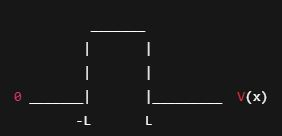
\includegraphics[width=0.4\textwidth]{Images/potential.JPG}}\label{fig:f1}
            \end{figure}

    \subsection{Solution, part (b):}
        We solve the time-independent Schrödinger equation:
        \[
            \frac{d^2\psi}{dx^2} + \frac{2m}{\hbar^2}(E - V(x))\psi = 0
        \]
        
        We define:
        \begin{itemize}
            \item Region I: \( x < -L \), where \( V(x) = 0 \)
            \item Region II: \( -L < x < L \), where \( V(x) = V_0 \)
            \item Region III: \( x > L \), where \( V(x) = 0 \)
        \end{itemize}
        
        Let \( E < V_0 \), so the particle is classically forbidden in Region II. Define:
        \[
            k = \sqrt{\frac{2mE}{\hbar^2}}, \qquad \kappa = \sqrt{\frac{2m(V_0 - E)}{\hbar^2}}
        \]
        
        Region I (\( x < -L \)):
        \[
            \psi_I(x) = A e^{k x}
            \quad \text{(only growing solution discarded as \( x \to -\infty \))}
        \]
        
        Region II (\( -L < x < L \)):
        \[
            \psi_{II}(x) = B \cosh(\kappa x) + C \sinh(\kappa x)
        \]
        
        Region III (\( x > L \)):
        \[
            \psi_{III}(x) = D e^{-k x}
            \quad \text{(only decaying solution allowed as \( x \to \infty \))}
        \]

    \subsection{Solution, part (c):}
        We apply the standard continuity conditions at \( x = \pm L \):
        \begin{align*}
            \psi_I(-L) &= \psi_{II}(-L) \\
            \psi'_I(-L) &= \psi'_{II}(-L) \\
            \psi_{II}(L) &= \psi_{III}(L) \\
            \psi'_{II}(L) &= \psi'_{III}(L)
        \end{align*}

        These equations allow solving for the constants \( A, B, C, D \) and determining allowed energies via a transcendental equation.

    \subsection{Solution, part (d):}
        Solve for the Case \( E < V_0 \). Even solution (symmetric), we assume:
        \[
            \psi_{II}(x) = B \cosh(\kappa x), \quad \psi_I(x) = A e^{k x}, \quad \psi_{III}(x) = A e^{-k x}
        \]
        
        Match boundary conditions at \( x = L \):
        \begin{align*}
            B \cosh(\kappa L) &= A e^{-k L} \\
            B \kappa \sinh(\kappa L) &= -A k e^{-k L}
        \end{align*}
        
        Divide:
        \[
            \frac{B \kappa \sinh(\kappa L)}{B \cosh(\kappa L)} = -k
            \quad \Rightarrow \quad \boxed{\kappa \tanh(\kappa L) = k}
        \]
        
        Odd solution (antisymmetric), we assume:
        \[
            \psi_{II}(x) = C \sinh(\kappa x), \quad \psi_I(x) = A e^{k x}, \quad \psi_{III}(x) = -A e^{-k x}
        \]
        
        Match boundary conditions at \( x = L \):
        \begin{align*}
            C \sinh(\kappa L) &= A e^{-k L} \\
            C \kappa \cosh(\kappa L) &= -A k e^{-k L}
        \end{align*}
        
        Divide:
        \[
            \frac{C \kappa \cosh(\kappa L)}{C \sinh(\kappa L)} = -k
            \quad \Rightarrow \quad \boxed{\kappa \coth(\kappa L) = k}
        \]

        Where:
        \[
            k = \sqrt{\frac{2mE}{\hbar^2}}, \qquad
            \kappa = \sqrt{\frac{2m(V_0 - E)}{\hbar^2}}
        \]

\section{Question 7}
    The Hamiltonian due to the interaction of a particle of mass \( m \), charge \( q \), and spin \( \vec{S} \) with a magnetic field pointing along the \( z \)-axis is
    \[
        \hat{H} = -\left( \frac{qB}{mc} \right) \hat{S}_z.
    \]
    
    Write the Heisenberg equations of motion for the time-dependent spin operators \( \hat{S}_x(t) \), \( \hat{S}_y(t) \), and \( \hat{S}_z(t) \), and solve them to obtain the operators as functions of time.

    \subsection{Solution:}
The Hamiltonian due to the interaction of a particle of mass \( m \), charge \( q \), and spin \( \vec{S} \) with a magnetic field pointing along the \( z \)-axis is
\[
\hat{H} = -\left( \frac{qB}{mc} \right) \hat{S}_z.
\]

In the Heisenberg picture, the time evolution of an operator \( \hat{A} \) is governed by:
\[
\frac{d\hat{A}}{dt} = \frac{i}{\hbar} [\hat{H}, \hat{A}]
\]

Using the spin commutation relations:
\[
[\hat{S}_i, \hat{S}_j] = i\hbar \epsilon_{ijk} \hat{S}_k
\]

Let \( \gamma = \frac{qB}{mc} \), then:
\[
\hat{H} = -\gamma \hat{S}_z
\]

We compute the time derivatives of the spin operators:
\begin{align*}
\frac{d\hat{S}_x}{dt} &= \frac{i}{\hbar} [-\gamma \hat{S}_z, \hat{S}_x] 
= -\gamma \frac{i}{\hbar} [\hat{S}_z, \hat{S}_x] 
= -\gamma \frac{i}{\hbar} (i\hbar \hat{S}_y) 
= \gamma \hat{S}_y \\
\frac{d\hat{S}_y}{dt} &= \frac{i}{\hbar} [-\gamma \hat{S}_z, \hat{S}_y] 
= -\gamma \frac{i}{\hbar} [\hat{S}_z, \hat{S}_y] 
= -\gamma \frac{i}{\hbar} (-i\hbar \hat{S}_x) 
= -\gamma \hat{S}_x \\
\frac{d\hat{S}_z}{dt} &= \frac{i}{\hbar} [-\gamma \hat{S}_z, \hat{S}_z] = 0
\end{align*}

From the above, we get the system:
\[
\begin{cases}
\frac{d\hat{S}_x}{dt} = \gamma \hat{S}_y \\
\frac{d\hat{S}_y}{dt} = -\gamma \hat{S}_x \\
\frac{d\hat{S}_z}{dt} = 0
\end{cases}
\]

Differentiate the first equation again:
\[
\frac{d^2\hat{S}_x}{dt^2} = \gamma \frac{d\hat{S}_y}{dt} = \gamma (-\gamma \hat{S}_x) = -\gamma^2 \hat{S}_x
\]
\[
\Rightarrow \frac{d^2\hat{S}_x}{dt^2} + \gamma^2 \hat{S}_x = 0
\]

This is a simple harmonic oscillator. The general solutions are:
\begin{align*}
\hat{S}_x(t) &= \hat{S}_x(0) \cos(\gamma t) + \hat{S}_y(0) \sin(\gamma t) \\
\hat{S}_y(t) &= \hat{S}_y(0) \cos(\gamma t) - \hat{S}_x(0) \sin(\gamma t) \\
\hat{S}_z(t) &= \hat{S}_z(0)
\end{align*}

This describes the precession of spin around the magnetic field direction (z-axis) at the Larmor frequency \( \gamma \).


\section{Question 8}
    \begin{enumerate}
        \item[(a)] Calculate the differential cross section in the Born approximation for the potential
        \[
        V(r) = V_0 \frac{e^{-r/R}}{r},
        \]
        known as the Yukawa potential.
    
        \item[(b)] Calculate the total cross section.
    
        \item[(c)] Find the relation between \( V_0 \) and \( R \) so that the Born approximation is valid.
    \end{enumerate}

    \subsection{Solution, part (a):}
        In the first Born approximation, the scattering amplitude is given by the Fourier transform of the potential:
        \[
            f(\mathbf{q}) = -\frac{2m}{\hbar^2} \cdot \frac{1}{4\pi} \int e^{i \mathbf{q} \cdot \mathbf{r}} V(r) \, d^3r
        \]
        
        For a spherically symmetric potential, this simplifies to:
        \[
            f(q) = -\frac{2m}{\hbar^2} \int_0^\infty r^2 \frac{\sin(qr)}{qr} V(r) \, dr
        \]
        
        Substituting the Yukawa potential:
        \[
            V(r) = V_0 \frac{e^{-r/R}}{r}
        \]
        \[
            f(q) = -\frac{2m V_0}{\hbar^2 q} \int_0^\infty e^{-r/R} \sin(qr) \, dr
        \]
        
        This is a standard integral:
        \[
            \int_0^\infty e^{-ar} \sin(br) \, dr = \frac{b}{a^2 + b^2}
            \qquad \text{with } a = \frac{1}{R}, \quad b = q
        \]
        
        So:
        \[
            f(q) = -\frac{2m V_0}{\hbar^2 q} \cdot \frac{q}{(1/R)^2 + q^2}
            = -\frac{2m V_0 R^2}{\hbar^2 (1 + q^2 R^2)}
        \]
        
        The differential cross section is then:
        \[
            \frac{d\sigma}{d\Omega} = |f(q)|^2 = \left( \frac{2m V_0 R^2}{\hbar^2 (1 + q^2 R^2)} \right)^2
        \]

    \subsection{Solution, part (b):}
        We integrate over the solid angle:
        \[
            \sigma = \int \frac{d\sigma}{d\Omega} d\Omega
            = \int_0^{2\pi} d\phi \int_0^\pi \left| f(q) \right|^2 \sin\theta \, d\theta
        \]
        
        Note that:
        \[
            q = 2k \sin\left( \frac{\theta}{2} \right)
        \]
        
        Therefore,
        \[
            \frac{d\sigma}{d\Omega} = \left( \frac{2m V_0 R^2}{\hbar^2 (1 + 4k^2 R^2 \sin^2(\theta/2))} \right)^2
        \]
        
        Now compute:
        \[
            \sigma = 2\pi \int_0^\pi \left( \frac{2m V_0 R^2}{\hbar^2 (1 + 4k^2 R^2 \sin^2(\theta/2))} \right)^2 \sin\theta \, d\theta
        \]
        
        Make the substitution \( u = \sin(\theta/2) \), so \( \sin\theta = 2u \sqrt{1 - u^2} \) and \( d\theta = \frac{2 du}{\sqrt{1 - u^2}} \). The integral becomes:
        \[
            \sigma = 8\pi \left( \frac{2m V_0 R^2}{\hbar^2} \right)^2 \int_0^1 \frac{u}{(1 + 4k^2 R^2 u^2)^2} \, du
        \]
        
        Let \( a = 4k^2 R^2 \), then:
        \[
        \int_0^1 \frac{x}{(1 + a x^2)^2} dx = \frac{1}{2a(1 + a)}
        \]
        
        Therefore:
        \[
        \sigma = 8\pi \left( \frac{2m V_0 R^2}{\hbar^2} \right)^2 \cdot \frac{1}{2a(1 + a)}
        = 8\pi \left( \frac{2m V_0 R^2}{\hbar^2} \right)^2 \cdot \frac{1}{8k^2 R^2 (1 + 4k^2 R^2)}
        \]
        
        Simplifying:
        \[
        \sigma = \frac{4\pi}{k^2} \left( \frac{m V_0 R}{\hbar^2 (1 + 4k^2 R^2)} \right)^2
        \]

    \subsection{Solution, part (c):}
        The Born approximation is valid when:
        \[
            \left| \frac{m}{\hbar^2 k} \int_0^\infty V(r) \sin(kr) r \, dr \right| \ll 1
        \]
        
        For the Yukawa potential:
        \[
            \left| \frac{m V_0}{\hbar^2 k} \int_0^\infty e^{-r/R} \sin(kr) \, dr \right|
            = \frac{m V_0}{\hbar^2 k} \cdot \frac{k}{k^2 + 1/R^2}
            = \frac{m V_0}{\hbar^2 (k^2 + 1/R^2)}
        \]
        
        Thus, the Born approximation is valid when:
        \[
            \frac{m V_0}{\hbar^2 (k^2 + 1/R^2)} \ll 1
        \]


\end{document}
